\documentclass[a4paper,14pt,twoside]{article}
\usepackage[german]{babel}
\usepackage[utf8]{inputenc}
\usepackage[T1]{fontenc}
\usepackage[svgnames]{xcolor}
\usepackage{amsmath, amsfonts, amssymb, graphicx, flafter, multirow, fancyhdr}
\usepackage[pdftex, colorlinks=true,linkcolor=DarkBlue, urlcolor=black, citecolor=DarkGreen]{hyperref}
\graphicspath{{./Bilder/}}
\usepackage{float}		%%zwingt Grafiken mit H genau an eingefügte Stelle
\pagestyle{fancy}
\fancyhf{}
\fancyhead[L]{{\small FOPRA - Physics Simulation with Geant4}}
%%\fancyhead[C]{{\small Lorenz Schlechter, \\Thomas Kraetzschmar}}
\fancyhead[R]{{\small\date{\today}}}
\fancyfoot[C]{\thepage}
\pagestyle{fancy}
\renewcommand{\topfraction}{0.9}
\renewcommand{\bottomfraction}{0.6}
\renewcommand{\textfraction}{0.1}
\setcounter{topnumber}{3}
% Title Page
\title{%
{\Huge Physics Simulation with Geant4}\\[0.5\baselineskip]
{\normalsize Gruppe 51}
}
\author{%
Thomas Kraetzschmar
\and Lorenz Schlechter
\and Maximilian Ziegler
}
\date{\today}
%#############################################################################
\begin{document}
\pagestyle{fancy}
\pagenumbering{roman}
\maketitle
\clearpage
%\cleardoublepage
\tableofcontents
\clearpage
\pagestyle{fancy}
\pagenumbering{arabic}
%*************************************************************************************
\section{Einleitung}
Simulationen spielen in vielen Bereichen der Physik und anderer Forschungsbereiche eine bedeutende Rolle, da mit einem vorher, in der Simulation; optimierten Aufbau viel Geld eingespart werden kann. Dank leistungsstarker Rechner und zunehmend optimierter Programme ist die Simulation hoch komplexer Vorgänge möglich. Dies hat zur Folge, dass nicht nur Aufbauten simuliert und optimiert werden, sondern auch Theorien überprüft werden können, in dem man die bei einem experimentellen Aufbau erhaltenen Ergebnisse mit den Theoretischen vergleicht.

Eines in der Physik verwendeten Simulationsprogramme ist Geant4. Mit diesem auf C++ basierenden Simulationssystem wurde während des Praktikumsversuches gearbeitet.

%--------------------------------------------------------------------------------------
\section{Introduction}

\section{Messung}
\subsection{Versuchsaufbau}
Um später die Genauigkeit der Simulation bestimmen zu können wurde zuerst der Simulierte Aufbau tatsächlich umgesetzt. Hierbei wurde eine Na-22 Quelle verqwendet. Diese zerfällt in einem $\beta^+$-Zerfall zu einem angeregten $^{22}Ne$, welches durch Emission eines Photons in den Grundzustand übergeht. Dieses Photon hat eine Energie von 1275 keV. Darüber hinaus kann das bei dem $\beta^+$-Zerfall entstandene Positron mit einem Hüllenelektron annihilieren, wobei zwei Photonen der Energie 511 keV entsehen.
Diese Photonen werden mittels Caesiumiodid Szintillationskristallen detektiert. \\\\Die Detektoren werden dabei auf vier verschiedene weisen platziert:
\begin{enumerate}
\item Die Quelle befindet sich in 3,5cm Höhe über dem Tisch, eine kleine Detektorbox befindet sich dabei in einem Abstand von 3cm, wobei der Detektorkristall sich 1cm tief in der Box befindet, der Gesamtabstand beträgt damit 4cm.
\item Gleicher Aufbau nur mit einem Abstand von 5cm bzw. einem Gesmatabstand von 6 cm.
\item Die Quelle befindet sich in 3,5cm Höhe und 3cm vor dem großen Detektor.
\item Die Quelle befindet sich in 3,5cm Höhe, auf der einen Seite befindet sich ein kleiner Detektor im Abstand von 5 cm, auf der anderen Seite ein kleiner Detektor über dem großen Detektor im gleichen Abstand.
\end{enumerate}
Die Messungen dauerten bei den ersten beidne Messungen 7 Minuten, bei der dritten 9 Minuten und bei dem vierten Aufbau 25 Minuten.


\subsection{Aktivität}
Die Aktivität der Probe wurde am 1.11.2013 zu $A_0=213 kBq$ bestimmt. Der Versuch wurde am 23.10.2014 durchgeführt, was einer Zeitdifferenz t von 357 Tagen entspricht. Die Halbwertszeit $T_{1/2}$ beträgt 2,6 Jahre. Damit beträgt die Aktivität zum Versuchszeitpunkt:
\begin{equation}
A=A_0*0,5^{t\over T_{1/2}}=164,11 kBq
\end{equation}


\subsection{Auswertung}
Die Messungen liefern die Anzahl der Ereignisse pro Kanal. Physikalisch interessant ist allerdings die Energie. Da die Energie der Peaks bekannt ist kann man daraus den Kanälen Energien zuordnen. Dies muss für jeden Kristall einmal durchgeführt werden. Bei der ersten Messung mit dem kleinen Kristall liegen die Peaks bei den Kanälen $4316,6\pm0,4$ und $10572\pm2$. Diese Entsprechen den Energien 511keV und 1275keV.
Damit lässt sich folgendermaßen eine Zuprdnung berechnen:
\begin{align}
E=m*K+t\\
m={{1275keV-511keV}\over{P_2-P_1}}\\
t=511keV-P_1*m
\end{align}
Wobei $P_1$ und $P_2$ die Postionen der Peaks sind.Daraus ergibt sich die Zuordnung:
\begin{equation}
E=0,12214*K-16,288
\end{equation}
Wobei K die Kanalnummer ist.
Dies ergibt bei der ersten Messung das in Abbildung \ref{l1} dargestellte Spektrum.
\begin{figure}[H]
	\begin{center}
	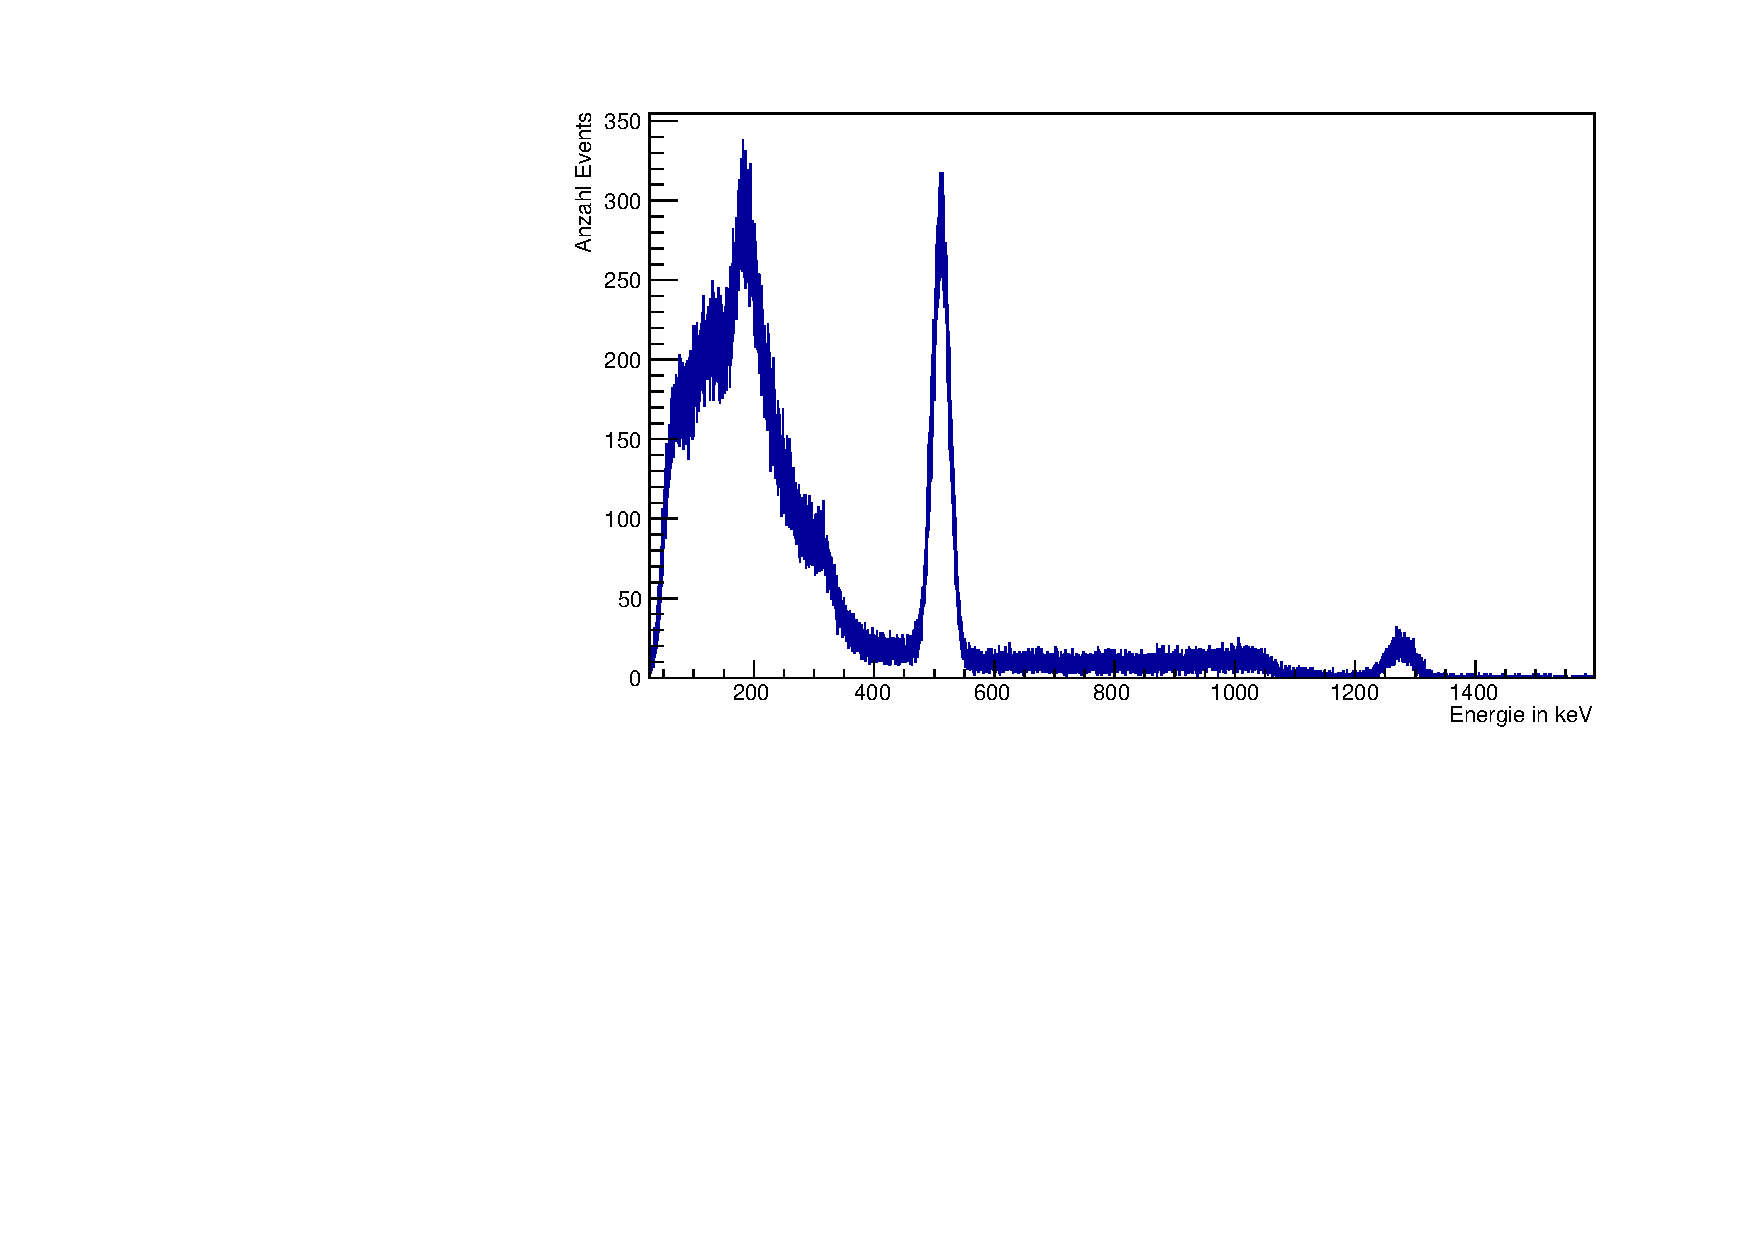
\includegraphics[width=0.7\linewidth]{Messung11.pdf}
	\caption{Spektrum der 1. Messung}
	\label{l1}
	\end{center}
\end{figure}
Um die Auflösung der Detektoren zu bestimmen werden die Peaks über eine Gaußkurve angenähert. Die Auflösung wird als die Halbwertsbreite definiert, die bei einer Normalverteilung bei 1,35$\sigma$ liegt. Bei der ersten Messung ergibt sich bei einem Fit von 470 keV bis 550 keV ein $\sigma$ von 15,77 keV. Ein Fit von 1200 keV bis 1350 keV liefert ein Sigma von 22,34 keV. Abbildung \ref{l2} zeigt den Fit des ersten Peaks. Damit ergibt sich eine Auflösung von 21,29keV bei 511 keV sowie von 30,15 keV bei 1275keV.
\begin{figure}[H]
	\begin{center}
	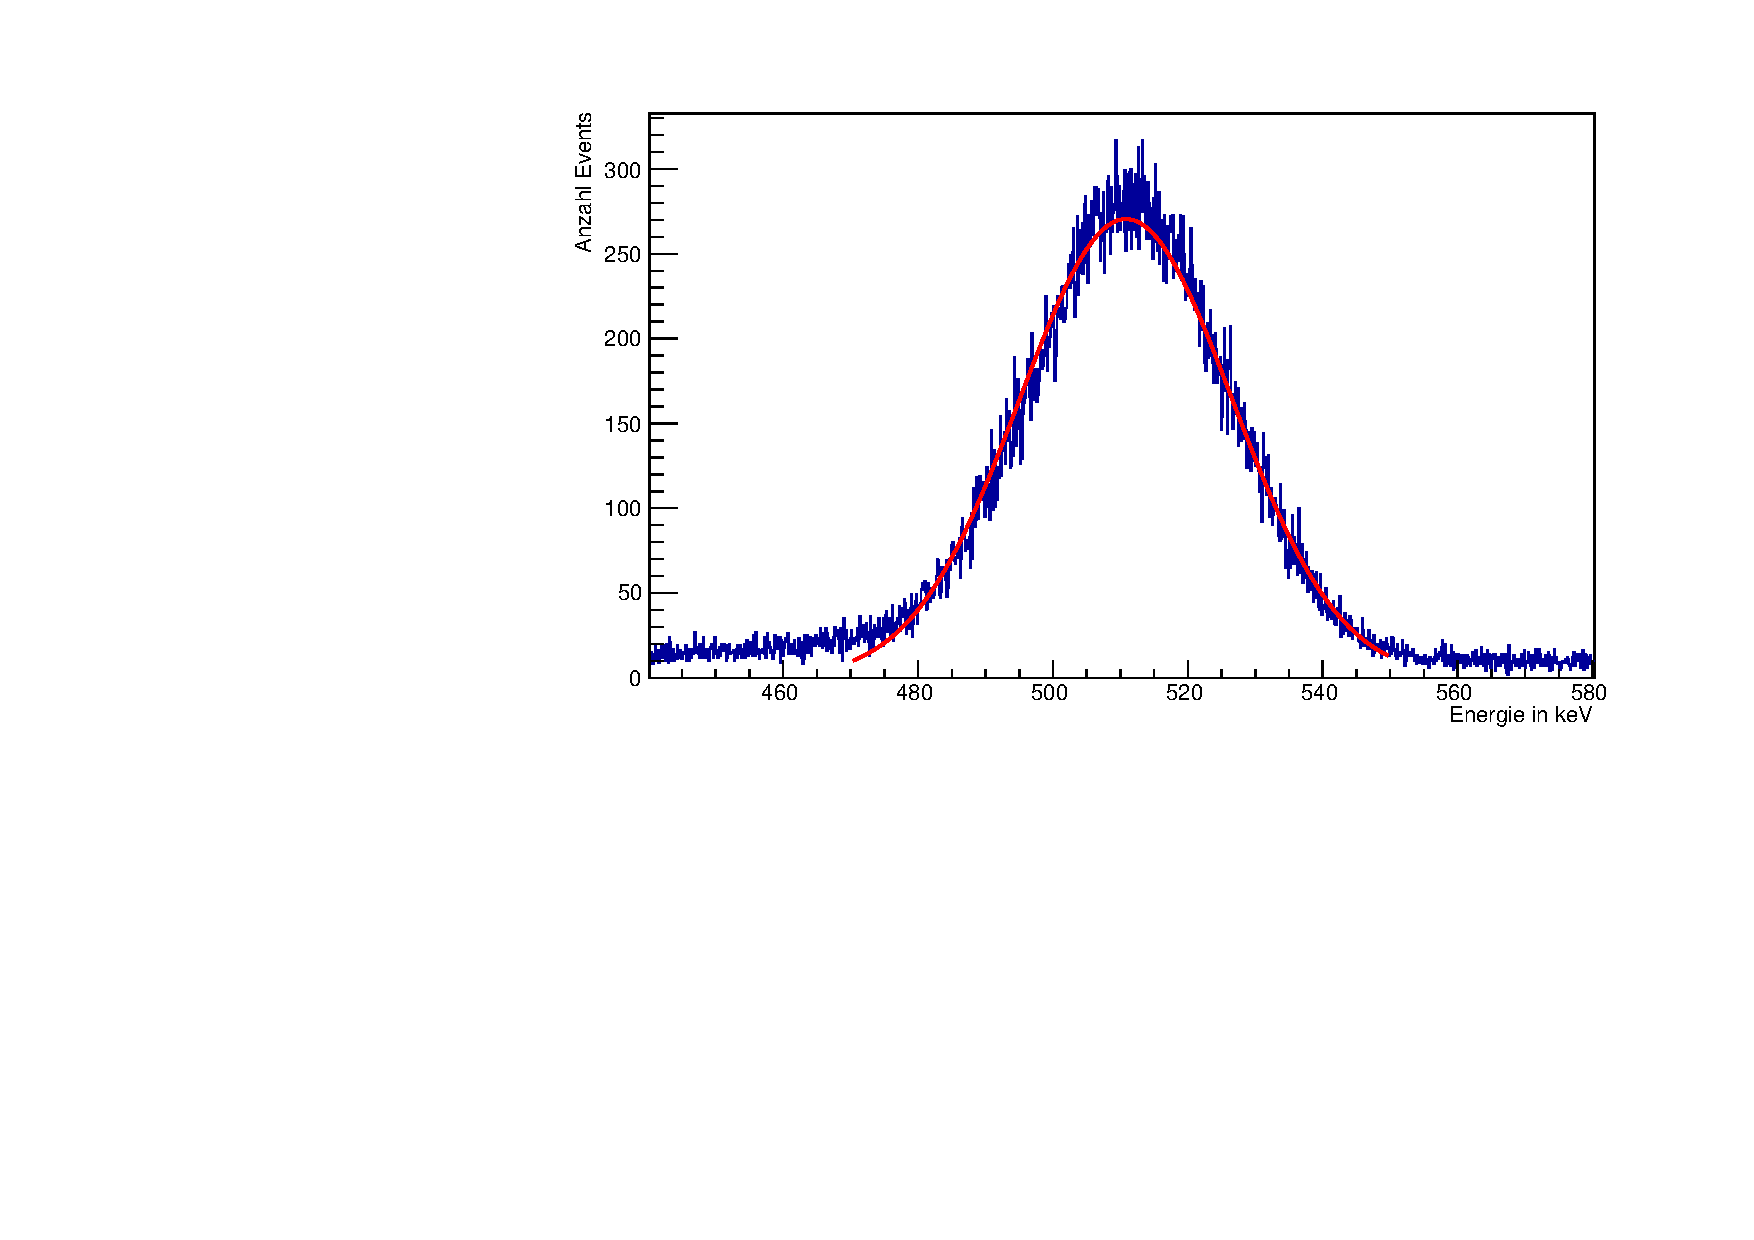
\includegraphics[width=0.7\linewidth]{Fit1.pdf}
	\caption{Gaußscher Fit des 511 keV Peaks der ersten Messung}
	\label{l2}
	\end{center}
\end{figure}
\ \\
\ \\
Die Effizienz setzt sich zusammen aus der geometrischen Effizienz und der Detektoreffizienz. Die geometrische Effizienz ist der Anteil des gesamten Raumwinkels den der Detektor abdeckt und wird über folgenden Ausdruck genähert:
\begin{equation}
\eta_{geometrisch}={A\over 4 \pi d^2}
\end{equation}
Die Photopeakeffizienz ergibt sich damit als
\begin{equation}
\eta_{Photopeak}={N_{peak}\over N_0\cdot\eta_{geometrisch}} \label{eq:Photopeak}
\end{equation}
Wobei $N_0$ die Anzahl der emitierten Photonen ist, die sich aus der Aktivität ergibt. Der kleine Detektor besteht aus einem Kristall der Frontfläche $A=11mm^2=121mm^2$. Der Wert für die Kirstalldimensionen wurde aus der Simulation ausgelesen. Bei der ersten Messung betrug der Abstand zur Detektorbox 3cm, der Gesamtabstand zwischen Quelle und Detektorkristall also 4cm. Damit ergibt sich eine geometrische Effizienz von 0,602\%. Zusammen mit der Aktivität von 164,11kBq sowie der Messzeit von 7 Minuten ergibt sich eine Photopeakffizienz von
\begin{equation}
\eta_{Photopeak}={87710\over 7\cdot60\cdot164110\cdot0,00602}=21,22\%
\end{equation}
Analog ergibt sich für die zweite Messung eine Auflösung von 20,91keV bzw 31,293keV und eine Effizienz von $\eta_{geometrisch}=0,096\%$ und $\eta_{Photopeak}=17,76\%$
Der große Kristall, der in Messung 3 und 4 verwendet wird, besteht aus zwei Kristallen. Die Eichung für diese ergibt die Gleichungen :
\begin {align}
E=0,473\cdot K-30,660\\
E=0,5922\cdot K-116,78
\end{align}
\\
Die beiden Kristalle haben eine Frontfläche A von $29 \cdot 13 mm^2=754mm^2$. Mit einem Gesamtabstand von 4 cm ergibt siche eine geometrische Effizienz von 3,75\%. Mit der Messdauer von 9 Minuten und 182430 Events ergibt sich eine Photopeakeffizienz von 7,06\%.
Die gaußschen Fits der Peaks liefern bei 511 keV eine über beide fits gemittelte Standardabweichung von 42,8keV bzw eine Auflösung von 57,77 keV.


\section{Reproduktion der Messungen}
	\subsection{Erster Aufbau}
		\subsubsection{Simulationsaufbau}
		Bei dieser Simulation wird versucht, die Messergebnisse des experimentellen Versuches mit dem Aufbau Nummer 1 zu reproduzieren. Die Programmierung hierzu war bereits geschehen und es muss nur noch die Simulation gestartet werden. Zur Simulation wird eine Anzahl von $10^6$ Events gewählt. 
		
		
		\subsubsection{Ergebnisse}
		Wie aus dem Spektrum (Abbildung (\ref{S1_ganz})) zu erkennen ist, repräsentiert die Simulation ziemlich gut die experimentellen Ergebnisse. Allerdings ist anzumerken, dass in einer zukünftigen Simulation deutlich mehr Events simuliert werden sollten, da die Peaks nur schwach ausgeprägt sind und das gesamt Spektrum sehr verschwommen ist, vor allem der 1.275 keV Peak ist nur erahnbar. Dies wurde in allen weiteren Simulationen berücksichtigt. 
		
		 
\begin{figure}[H]
	\begin{center}
		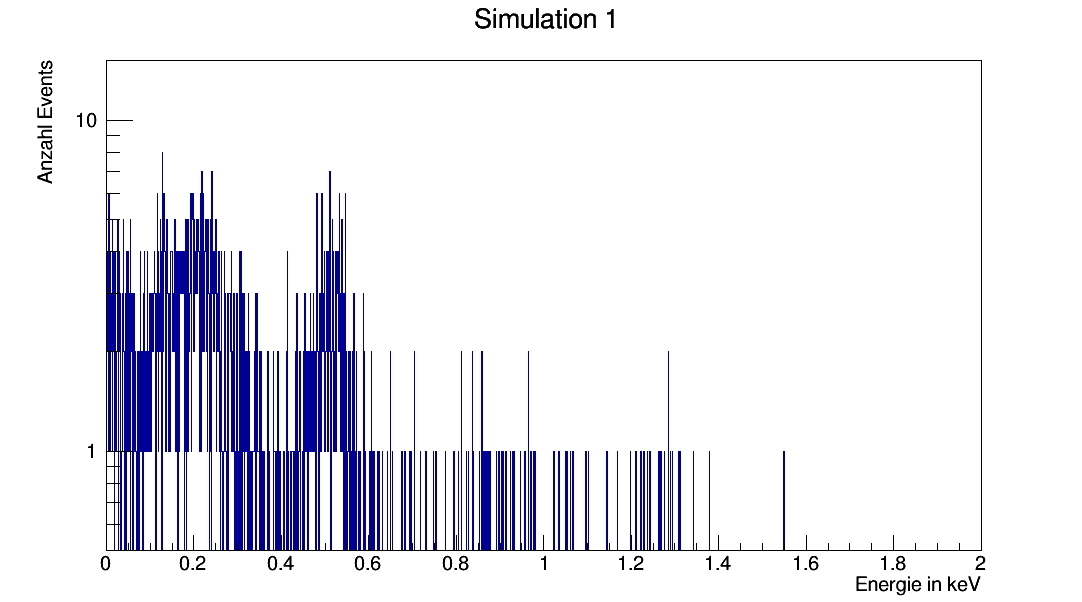
\includegraphics[width=0.7\linewidth]{Simulation1_ganz}
		\caption{Spektrum der ersten Simulation}
		\label{S1_ganz}
	\end{center}
\end{figure}	

Für die Berechnung der Effizienz wird folgende Formel verwendet:
\begin{align}
	\epsilon = \frac{N_{\textrm{peak}}}{N}
\end{align}
Wobei $N_\textrm{peak}$ die Anzahl der Events, die in dem entsprechenden Peak stattfinden und N die gesamte Anzahl an Events entspricht, die in der Simulation berechnet wurden. Somit ergibt sich eine Effizienz von $(3.27\cdot 10^{-2}\%$ des Peaks bei 511 eV (ermittelt: $(508\pm 9)$eV)  und $(1.8\cdot 10^{-3}\%$ des Peaks bei 1275 eV (ermittelt: $(1.29\pm 0.03)$keV). Die hierbei verwendeten Werte wurden durch einen Gauss-Fit ermittelt, wofür hier exemplarisch der Fit für den 511 eV Peak in der Abbildung (\ref{S1_511_fit}) abgebildet ist. Für die Berechnung der Anzahl der Events wurde die FWHM Verteilung verwendet. Insgesamt ergibt sich eine Photopeak-Effizienz von $\mu_\textrm{Photopeak 511eV}=5.43\cdot 10^{-2} \% $ und $\mu_\textrm{Photopeak 1275eV}=2.9\cdot 10^{-3} \% $. Diese berechnet sich analog mit Formel (\ref{eq:Photopeak}). Die Auflösung des Detektors berechnet sich analog zu den experimentellen Versuchen und betragen somit 171 eV bei 511 eV und 91 eV bei 1275 eV.
		
\begin{figure}[H]
	\begin{center}
		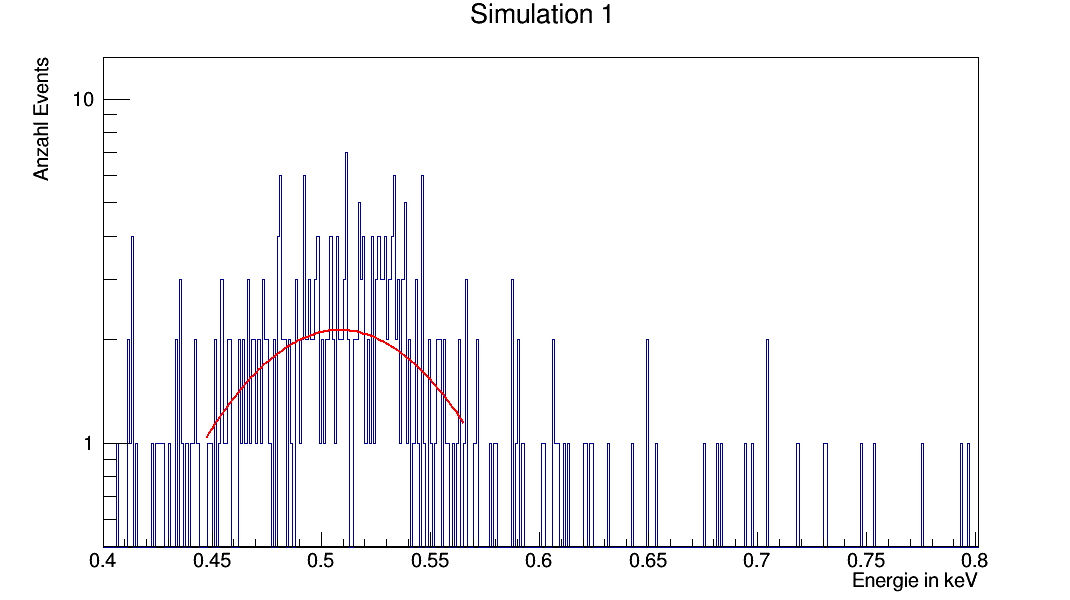
\includegraphics[width=0.7\linewidth]{Simulation1_511_fit}
		\caption{Fit des Peaks bei 511eV}
		\label{S1_511_fit}
	\end{center}
\end{figure}		
		
		
		
	\subsection{Aufbau Nummer 3}
		\subsubsection{Simulationsaufbau}
			Um diesen Aufbau nachzubilden, muss eine weitere Box implementiert werden. Diese hat folgende Ausmaße (100x81x200mm$^3$) mit einer Dicke von 6mm, so dass zwei Kristalle mit dem Volumen 29x13x130mm$^3$ darin übereinander platziert werden können. Es werden $10^7$ Events simuliert. Alle Abstände sind wie in dem entsprechenden Versuch. 
			
		\subsubsection{Ergebnisse}
			Bei dieser Simulation werden insgesamt 3 verschiedene Spektren aufgenommen. Es werden beispielhaft hier nur die Abbildungen des 1. Kristalls in der großen Box verwendet, alle weiteren Abbildungen befinden sich im Anhang.
			Auch hierfür können die jeweiligen Effizienzen analog berechnet werden. Diese betragen: \\
			\begin{figure}[H]
			\begin{center}
			
			
			\begin{tabular}{|c|c|c|c|}
			\hline 
			\rule[-1ex]{0pt}{2.5ex} Kristall & $\epsilon$ & Photopeak-Effizienz & Auflösung [eV]\\ 
			\hline 
			\rule[-1ex]{0pt}{2.5ex} kleiner 511 eV & $1.32\cdot 10^{-2}\%$ & $2.19\cdot 10^{-2}\%$ & $(93.3\pm 1.9)$ \\ 
			\hline 
			\rule[-1ex]{0pt}{2.5ex} kleiner 1275 eV & $1.44\cdot 10^{-3}\%$ & $2.39\cdot 10^{-3}\%$ &  $(268.4\pm 509.2)$\\ 
			\hline 
			\rule[-1ex]{0pt}{2.5ex} 1. Kristall (große Box) 511 eV &  $3.77\cdot 10^{-2}\%$ & $1.01\cdot 10^{-2}\%$ & $(43.1\pm 47.2 )$\\ 
			\hline 
			\rule[-1ex]{0pt}{2.5ex} 1. Kristall (große Box) 1275 eV & $8.98\cdot 10^{-3}\%$ & $2.39\cdot 10^{-3}\%$ & $(174.8\pm 10.8)$ \\ 
			\hline 
			\rule[-1ex]{0pt}{2.5ex} 2. Kristall (große Box) 511 eV & $3.70\cdot 10^{-2}\%$ & $1.01\cdot 10^{-2}\%$ & $(136.2\pm 51.4)$ \\ 
			\hline 
			\rule[-1ex]{0pt}{2.5ex} 2. Kristall (große Box) 1275 eV & $9.3\cdot 10^{-3}\%$ & $2.48\cdot 10^{-3}\%$ & $(187.0\pm 14.1)$ \\ 
			\hline 
			\end{tabular}
			\end{center}
			\caption{Effizienzen der Kristalle}
			\end{figure}
			
			Auch hier ist wieder anzumerken, dass die Fehler in der Auflösung deutlich reduziert werden könnten, wenn mehr Events für diese Simulation berechnet werden. Vor allem bei dem Fit des Peaks bei 1275 eV des kleinen Kristalls (Abbildung (\ref{S2_1275_fit})) wird dies extrem sichtbar. 
			
			
			\begin{figure}[H]
				\begin{center}
				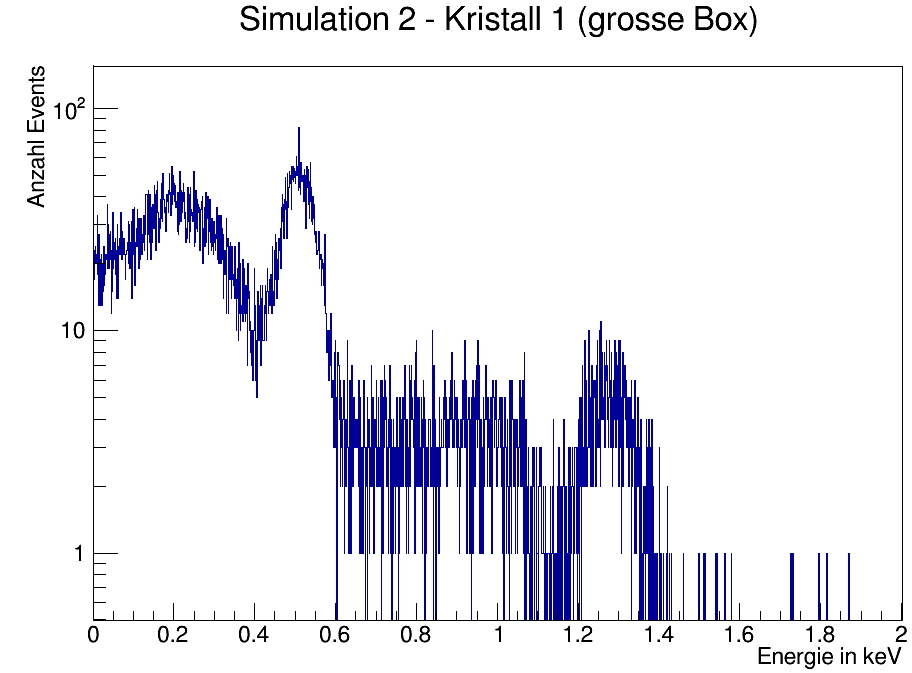
\includegraphics[width=0.7\linewidth]{Simulation2(1KGB)_ganz}
				\caption{Spektrum des 1. Kristall in der großen Box}
				\label{S2_1KGB_ganz}
				\end{center}
			\end{figure}
			
			\begin{figure}[H]
				\begin{center}
				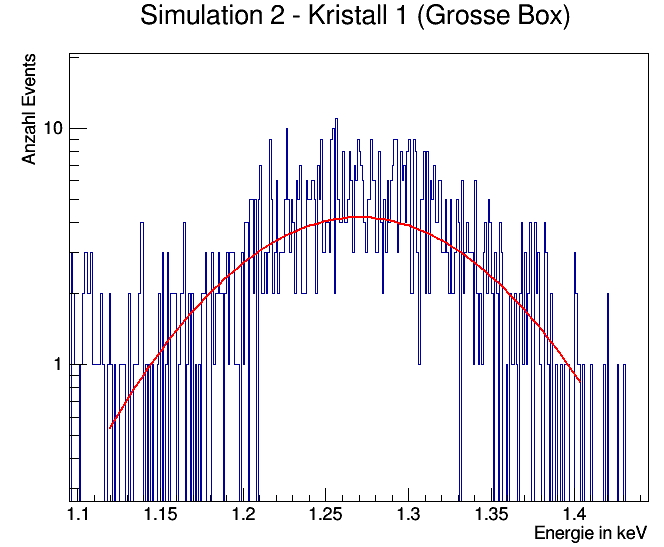
\includegraphics[width=0.7\linewidth]{Simulation2(1KGB)_1275_fit}
				\caption{Fit des Peaks bei 1275 eV}
				\label{S2_1KGB_1275_fit}
				\end{center}
			\end{figure}
			 
	\subsection{Aufbau Nummer 3 mit Germanium}
		\subsubsection{Simulationsaufbau}
			Es wird der selbe Aufbau wie bei der Simulation zuvor verwendet. Allerdings wird das CsI des Detektors durch Ge ersetzt um die verschiedenen Einflüsse der Materialien zu testen.
			
			
		\subsubsection{Ergebnisse}
			Im direkten Vergleich zwischen den Spektren der Abbildungen (\ref{S3_ganz}) und (\ref{S2_KB_ganz}) lässt bereits erkennen, dass Ge-Kristall eine höhere Effizienz hat als der CsI-Kristall.
			
			\begin{figure}[H]
				\begin{center}
				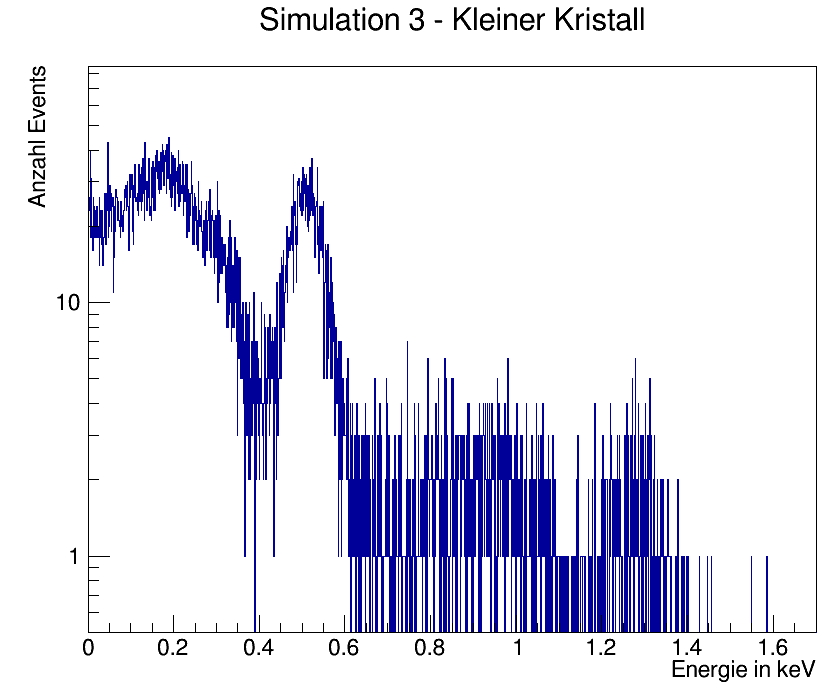
\includegraphics[width=0.7\linewidth]{Simulation3(KB)_ganz}
				\caption{Spektrum des kleinen Kristalls}
				\label{S3_ganz}
				\end{center}
			\end{figure}
			
			Diese erste Annahme wird auch durch die Berechnung der jeweiligen Effizienzen für die Peaks bestätigt, wobei $\epsilon_\textrm{511 eV}=2.67\cdot 10^{-2}\%$ und $\epsilon_\textrm{1275 eV}=5.44\cdot 10^{-3}\%$.  Für die Photopeak-Effizienzen gilt somit:$\mu_\textrm{Photopeak 511 eV}=4.44\cdot 10^{-2}\%$ und $\mu_\textrm{Photopeak 1275 eV}=9.04\cdot 10^{-3}\%$. Dies entspricht im Falle des 511 eV Peaks ca dem doppelten des entsprechenden Wertes aus Simulation 2. Im Falle des 1275 eV Peaks sogar dem 3.8 fachen. Für die Berechnung der Auflösung gilt wieder die FWHM Verteilung. Somit ergeben sich folgende Auflösungen: $(93.8\pm 1.2)$ eV bei dem 511 eV Peak und $(330.6\pm 85.2)$ eV bei dem 1275 Peak. Die hierfür verwendeten Fits finden sich in den Abbildungen (\ref{S3_511_fit}) und (\ref{S3_1275_fit}). Betrachtet man allerdings die Auflösungen der zwei unterschiedlichen Materialien ist der Unterschied vernachlässigbar klein. 
			
			\begin{figure}[H]
				\begin{center}
				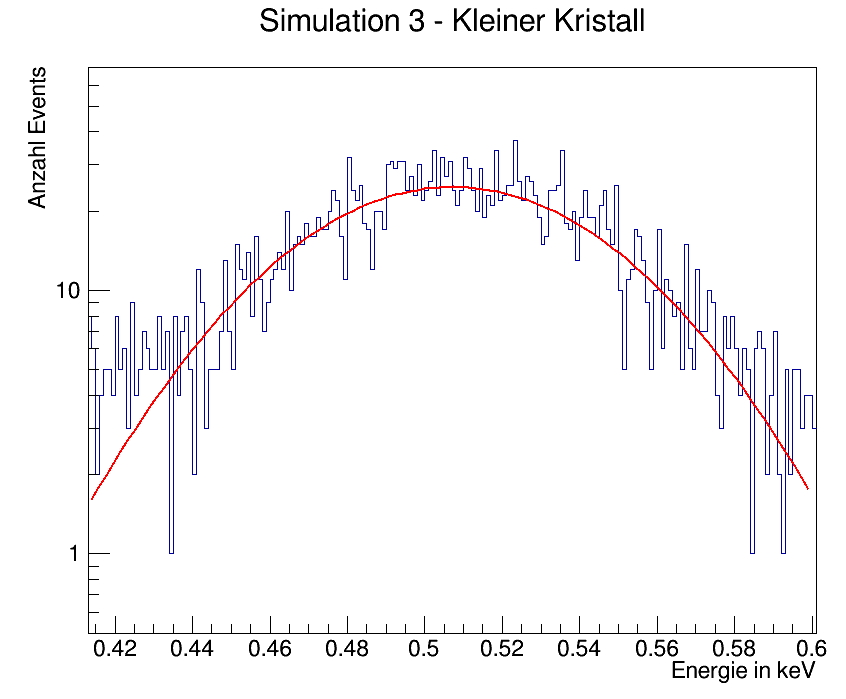
\includegraphics[width=0.7\linewidth]{Simulation3(KB)_511_fit}
				\caption{Fit des Peaks bei 511 eV}
				\label{S3_511_fit}
				\end{center}
			\end{figure}
			
			\begin{figure}[H]
				\begin{center}
				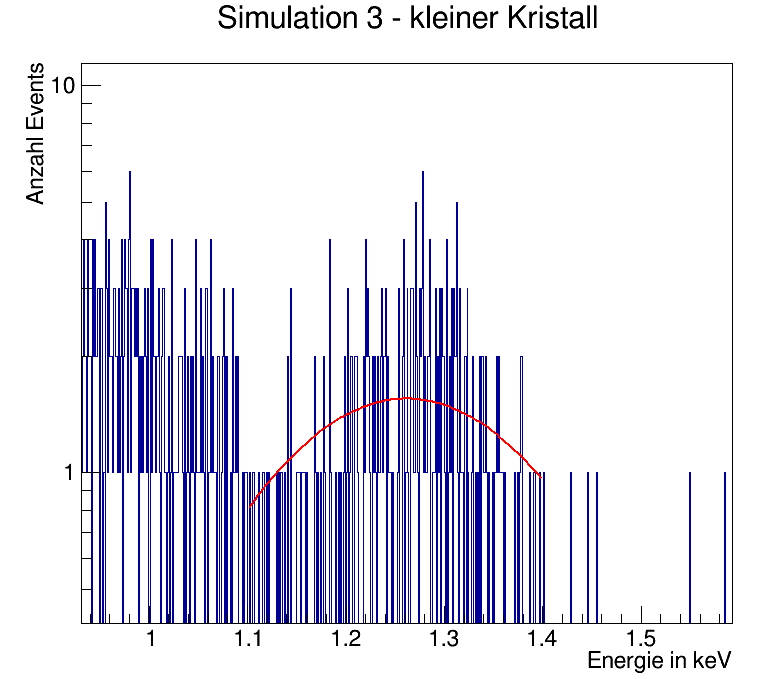
\includegraphics[width=0.7\linewidth]{Simulation3(KB)_1275_fit}
				\caption{Fit des Peaks bei 1275 eV}
				\label{S3_1275_fit}
				\end{center}
			\end{figure}
			
\section{Entwicklung eines Detektorsystems}
	\subsection{4, 8, 20 Detektor-Elemente}			
		\subsubsection{Simulationsbeschreibung}
			Nun soll der Detektor so designed werden, dass er symmetrisch um den $\gamma$ (1MeV) Strahl (hier in Zeichenebene) aufgebaut ist. Dieser Ionen Strahl wird mit dem Doppler Effekt behandelt ($\beta=0.7$). Die Kristalle haben alle die Ausmaße von 2x2x15cm$^3$ und sind ummantelt mit einer dünnen (1mm) Al-Box. Die $\gamma$ Quelle befindet sich 30cm vor dem Detektor. Angeordnet sollen die einzelnen Kristalle, wie in Abbildung (\ref{fig:Aufbau}) beschrieben, werden. Es werden jeweils wieder 10$^7$ Events simuliert. 
			
			\begin{figure}[H]
				\begin{center}
				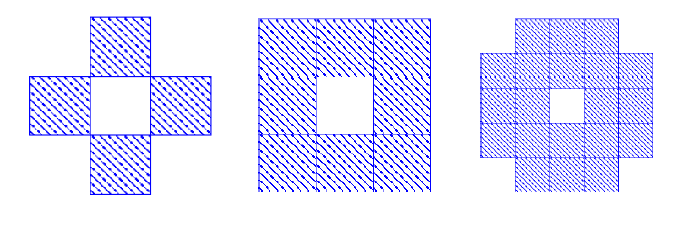
\includegraphics[width=0.7\linewidth]{Aufbau}
				\caption{Aufbau des Detektors mit 4,8,20 Kristallen}
				\label{fig:Aufbau}
				\end{center}
			\end{figure}


		\subsubsection{Ergebnisse}
			{\color{Red} Noch einzufügen}
			
			
			
			
			
			
	\subsection{32 Detektor-Elemente}
		\subsubsection{Simulationsaufbau}
			In dieser Simulation wird die Höhe und Breite der Kristalle halbiert, somit haben sie nur noch eine Ausdehnung von 1x1x15cm$^3$. Jeder Kristall ist wieder von einer 1mm dicken Al-Box umgeben. Angeordnet sollen die Kristalle so, dass sie dieselbe Fläche einnehmen wie das 8-Kristalle Setup aus der letzten Simulation. 
			
			
			
		\subsubsection{Ergebnisse}
			{\color{Red} Noch einzufügen}
			
			
			
	\subsection{Evaluation der Kosten}
		{\color{Red} Noch einzufügen}
		
		
		
	\subsection{Entscheidung bei bestimmten Vorgaben}
		{\color{Red} Noch einzufügen}

			
\section{Anhang}
	\subsection{Abbildungen}
	
\begin{figure}[H]
	\begin{center}
		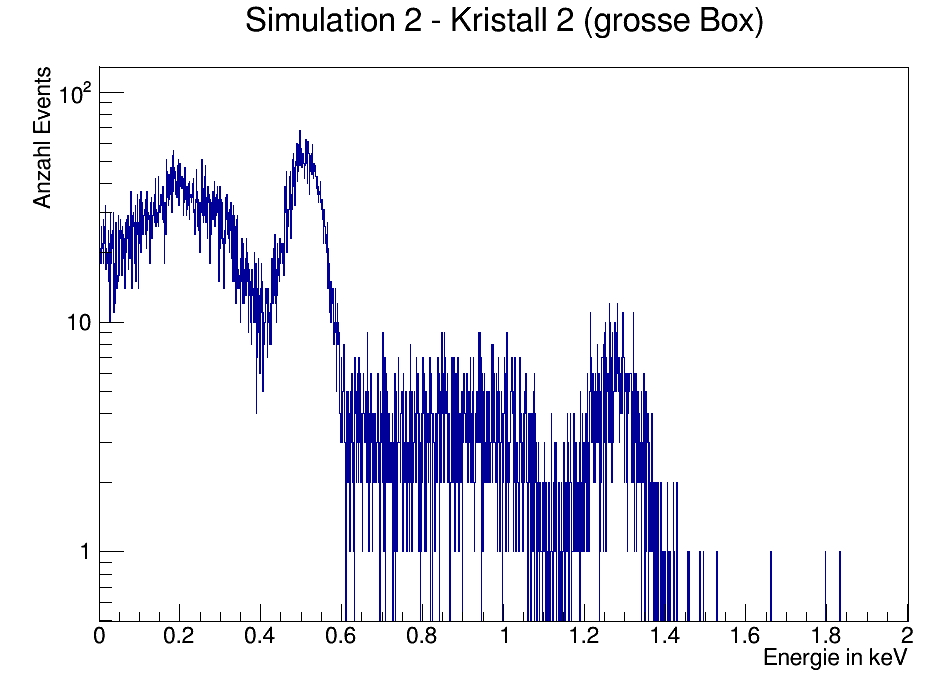
\includegraphics[width=0.7\linewidth]{Simulation2(2KGB)_ganz}
		\caption{Spektrum des 2. Kristalls in der großen Box}
		\label{}
	\end{center}
\end{figure}

\begin{figure}[H]
	\begin{center}
		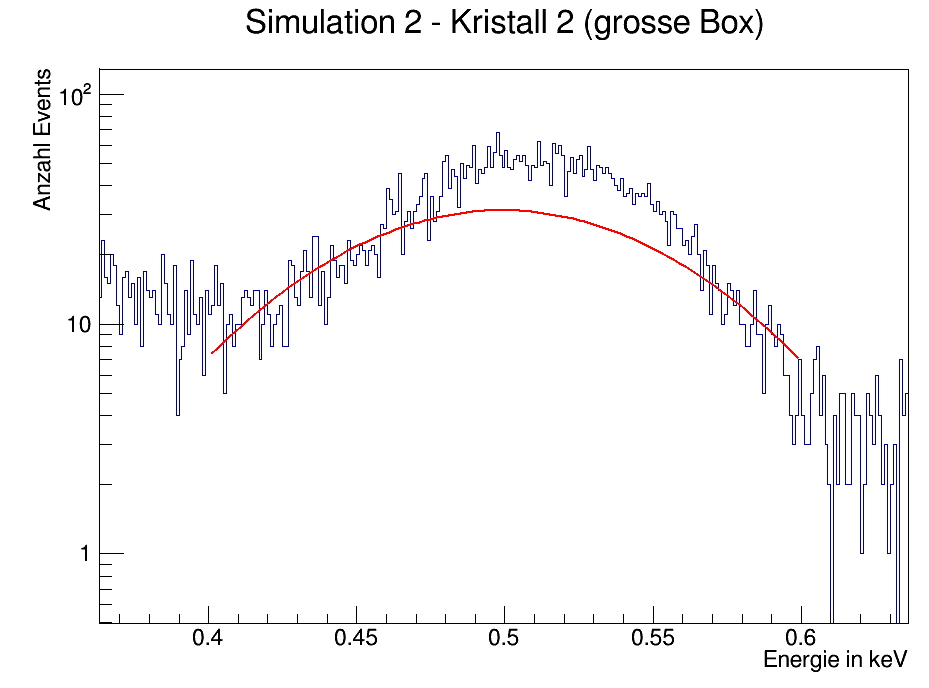
\includegraphics[width=0.7\linewidth]{Simulation2(2KGB)_511_fitt}
		\caption{Fit des Peaks bei 511 eV des 2.Kristalls der großen Box}
		\label{}
	\end{center}
\end{figure}

\begin{figure}[H]
	\begin{center}
		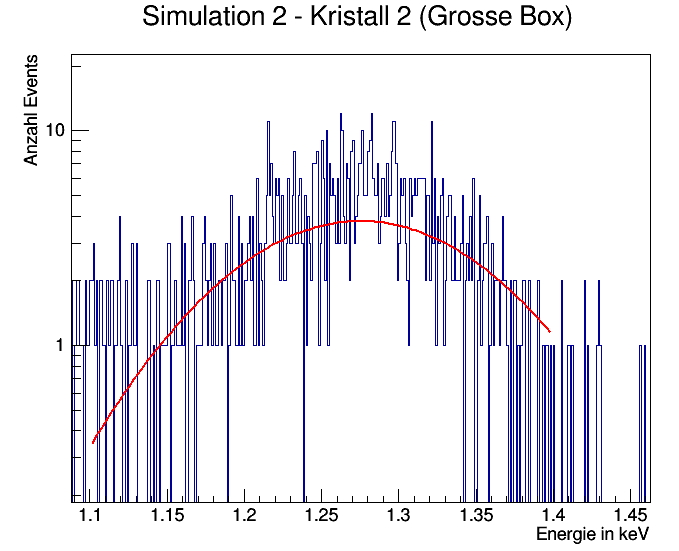
\includegraphics[width=0.7\linewidth]{Simulation2(2KGB)_1275_fitt}
		\caption{Fit des Peaks bei 1275 eV des 2.Kristalls der großen Box}
		\label{}
	\end{center}
\end{figure}

\begin{figure}[H]
	\begin{center}
		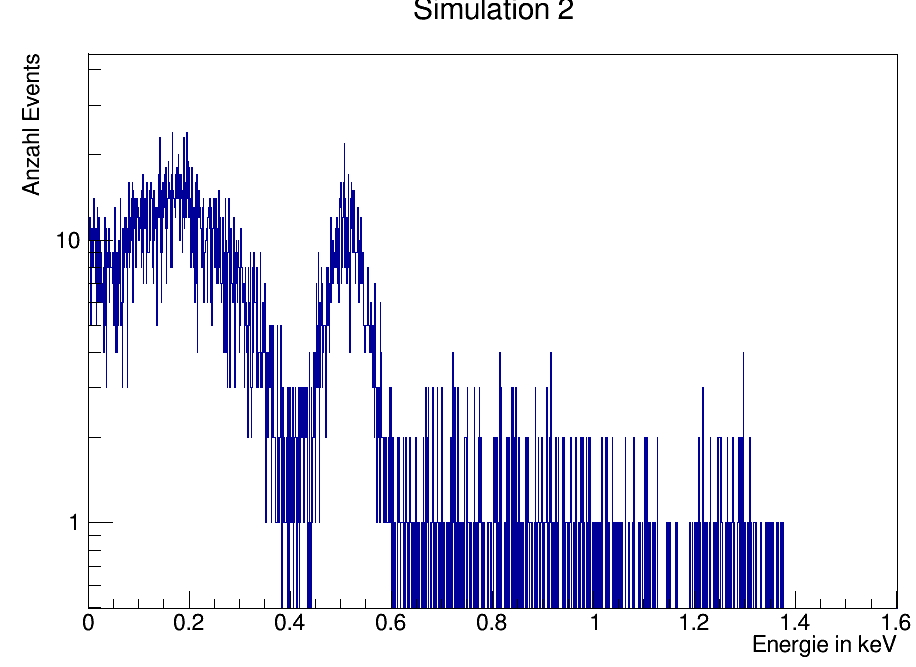
\includegraphics[width=0.7\linewidth]{Simulation2_ganz}
		\caption{Spektrum des kleinen Kristalls}
		\label{S2_KB_ganz}
	\end{center}
\end{figure}

\begin{figure}[H]
	\begin{center}
		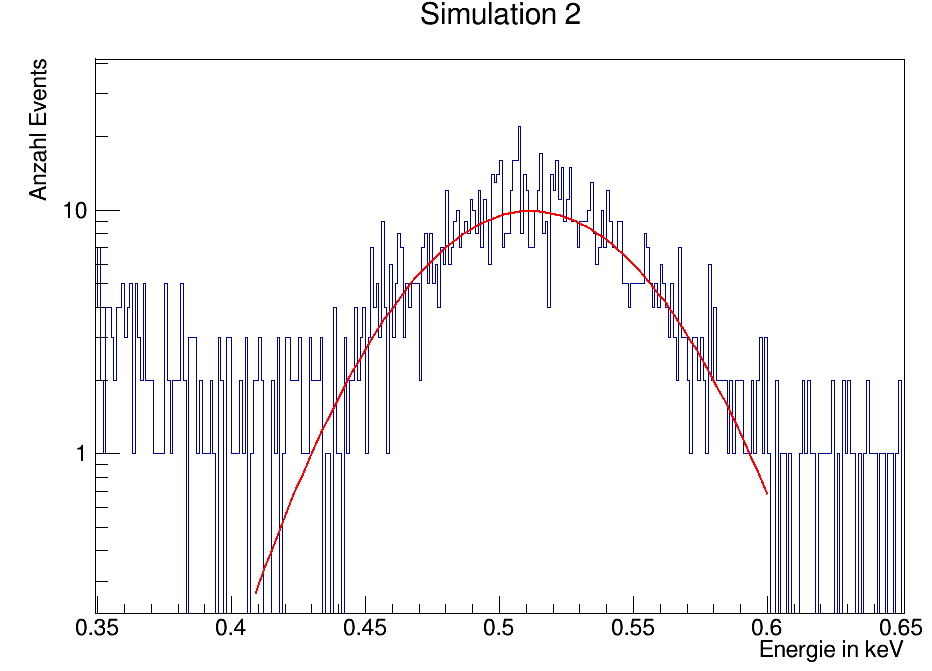
\includegraphics[width=0.7\linewidth]{Simulation2_511_fit}
		\caption{Fit des Peaks bei 511 eV des kleinen Kristalls}
		\label{}
	\end{center}
\end{figure}

\begin{figure}[H]
	\begin{center}
		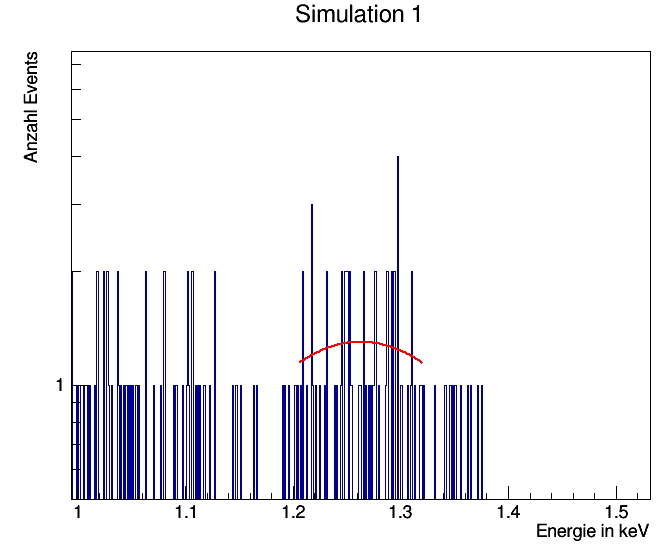
\includegraphics[width=0.7\linewidth]{Simulation2_1275_fit}
		\caption{Fit des Peaks bei 1275 eV des kleinen Kristalls}
		\label{S2_1275_fit}
	\end{center}
\end{figure}


		
	\subsection{Literaturverzeichnis}
		Alle Formeln, Abbildungen und nahezu alle Aussagen sind der Versuchsanleitung zu entnehmen. 
	Sonst wurde keine weitere Literatur verwendet.\\
	\url{https://www.ph.tum.de/academics/org/labs/fopra/docs/userguide-77.en.pdf} \\
	
%\bibliographystyle{alpha}
%\bibliographystyle{apalike}
%\bibliographystyle{plain}
%\bibliography{Literaturverzeichniss-Brue}
%\appendix
%\listoffigures
%\listoftables
%
\end{document} 